
\chapter{Алгоритмы приближенного решения задачи Коши для ОДУ}\label{ch-ODE}

\section{Общие сведения}
Пространством Соболева $W^r_{L^{2}_\rho}$  назовем класс функций $f$, непрерывно дифференциируемых $r-1$-раз, причем $f^{(r-1)}$ абсолютно непрерывна, а $f^{(r-1)}\in L^2_\rho(a,b)$. Скалярное произведение функций $f,g\in W^r_{L^{2}_\rho}$ типа Соболева определяется следующим равенством
\begin{equation*}
  \langle f,g\rangle = \sum\limits_{\nu=0}^{r-1}f^{(\nu)}(a)g^{(\nu)}(a)+\int\limits_a^b f^{(r)}(x)g^{(r)}(x)\rho(x)dx.
\end{equation*}
Характерной особенностью скалярных  произведений типа Соболева является, в частности, то, что они, как правило,  содержат слагаемые, которые <<контролируют>> поведение соответствующих ортогональных полиномов в одной или нескольких точках числовой оси.


\section{Быстрый алгоритм приближенного нахождения решения задачи Коши для ОДУ посредством соболевских функций, порожденных косинусами}


В данном подразделе рассмотрен алгоритм быстрого приближенного нахождения решения задачи Коши для ОДУ путем вычисления коэффициентов разложения этого решения в ряд по системе функций $\{\varphi_{1,n}(x)\}_{n=0}^{\infty}$, где $ \varphi_{1,0}(x)=1$, $\varphi_{1,1}(x)=x$, $\varphi_{1,n+1}(x)=\frac{\sqrt{2}}{\pi n}\sin(\pi nx)$, $n=1,2,\ldots$,
ортонормированной относительно скалярного произведения Соболева $\langle f, g\rangle=f(0)g(0)+\int_0^1f'(x)g'(x)dx$ и порожденной
косинусами $\varphi_0(x)=1,\ \{\varphi_n(x)=\sqrt{2}\cos(\pi nx)\}_{n=1}^\infty$.
Вычисление коэффициентов осуществляется посредством итерационного процесса с применением быстрого преобразования Фурье на каждой итерации.


\subsection{Введение}

В работе \cite{RamShaMag} была введена система функций
\begin{equation}\label{GasRam-eq1}
 \varphi_{1,0}(x)=1,\quad \varphi_{1,1}(x)=x,\quad \varphi_{1,n+1}(x)=\frac{\sqrt{2}}{\pi n}\sin(\pi nx),\quad n=1,2,\ldots,
\end{equation}
которая ортонормирована относительно скалярного произведения Соболева
\begin{equation*}
\langle\varphi_{1,n},\varphi_{1,m}\rangle=\varphi_{1,n}(0)\varphi_{1,m}(0)+\int_0^1\varphi'_{1,n}(x)\varphi'_{1,m}(x)dx
\end{equation*}
и порождена системой косинусов
\begin{equation}\label{GasRam-eq2}
\varphi_0(x)=1,\quad \{\varphi_n(x)=\sqrt{2}\cos(\pi nx)\}_{n=1}^\infty
\end{equation}
посредством равенств
$$
 \varphi_{1,0}(x)=1,\quad \varphi_{1,n}(x)=\int_0^x \varphi_{n-1}(t)dt, \quad n=1,2,\ldots
$$

В этой же работе было показано, что системы \eqref{GasRam-eq1} и \eqref{GasRam-eq2}, взятые вместе являются весьма эффективным инструментом численного решения систем линейных и нелинейных дифференциальных уравнений с помощью итерационного процесса, основанного на построении сжимающего оператора $A$. С подробным описанием этого итерационого процесса и построением сжимающего оператора можно ознакомиться в работе \cite{RamSharDemr}. В данном подразделе мы рассмотрим задачу Коши
\begin{equation}\label{GasRamequCau}
y{'} = f(x,y), \quad y(0) = y^0, \quad x \in [0, h],
\end{equation}
где $h$ выбирается из условия \eqref{GasRamconditionfor_h}, $f(x,y)$ --- функция двух переменных, которая непрерывна в некоторой замкнутой области $\bar{G}$ переменных $(x,y)$, содержащей точку $(0,y^0)$ и такой, что  $[0,h]\times\mathbb{R}\subset\bar G$.
Кроме того, функция $f(x,y)$ удовлетворяет условию Липшица по второй переменной, т.е.
\begin{equation*}
 \left|f(x,y_{1})-f(x,y_{2})\right|\leq\lambda\left|y_{1}-y_{2}\right|,\quad0\leq x\leq h.
\end{equation*}
Выполнив замену переменной $x = h\sin \pi t$ в \eqref{GasRamequCau}, мы перейдем к следующей задаче
\begin{equation}\label{GasRamequafterrep}
\eta{'}(t) = h\pi \cos(\pi t) f(h\sin \pi t, \eta(t)), \quad \eta(0) = y^0, \quad 0 \leq t \leq \frac{1}{2},
\end{equation}
где
$\eta(t)=y(h\sin \pi t)$. Заметим, что после такой замены функция $y(h\sin \pi t)$ на отрезке $[0,1]$ будет симметричной относительно прямой $t=\frac{1}{2}$. Поэтому в дальнейшем мы будем считать, что $t\in[0,1]$.
Так как функция $f(x,y)$ непрерывна в области $\bar{G}$, то $\eta(t)\in W^1_{L^2(0,1)}$. Тогда в силу теоремы 2.2 из работы \cite{RamShaIzv} следует, что функцию  $\eta(t)$ можно разложить в равномерно сходящийся ряд Фурье по системе \eqref{GasRam-eq1}, т.е.
\begin{equation}\label{GasRamFourierserforg}
\eta(t) = \eta(0)+\sum_{k=0}^\infty c_{1,k+1}(\eta)\varphi_{1,k+1}(t),
\end{equation}
где
$$
c_{1,k+1}(\eta)=\int\limits_0^1\eta{'}(\tau)\varphi_k(\tau)d\tau.
$$
Кроме того, в силу полноты системы \eqref{GasRam-eq2} в $L^2(0,1)$, для функций $\eta{'}(t)$ и \linebreak$q(t)=\cos(\pi t) f(h\sin \pi t, \eta(t))$ в метрике пространства $L^2(0,1)$, имеют место следующие разложения в ряд Фурье по системе \eqref{GasRam-eq2}:
\begin{equation}\label{GasRamg-Fourser}
\eta{'}(t) =  \sum_{k=0}^\infty c_{1,k+1}(\eta)\varphi_k(t),
\end{equation}
\begin{equation}\label{GasRamq-Fourser}
q(t)=\cos(\pi t) f(h\sin \pi t,\eta(t)) = \sum_{k=0}^\infty c_{k}(q)\varphi_k(t).
\end{equation}
Тогда из \eqref{GasRamequafterrep}--\eqref{GasRamq-Fourser} для $k\geq0$ имеем
$$
c_{1,k+1}(\eta)=h\pi c_{k}(q)=h\pi\int\limits_0^1 f(h\sin \pi \tau,\eta(\tau))\cos(\pi \tau)\varphi_k(\tau)d\tau=
$$
$$
h\pi\int\limits_0^1 f\left(h\sin \pi \tau, \eta(0)+\sum_{i=0}^\infty c_{1,i+1}(\eta)\varphi_{1,i+1}(\tau)\right)\cos(\pi \tau)\varphi_k(\tau)d\tau.
$$
Правая часть последнего равенства и есть вышеупомянутый оператор $A$, сопоставляющий точке $(c_0,c_1, \ldots)\in l^2$ точку $(c'_0,c'_1, \ldots)\in l^2$ по правилу
$$
c'_k=h\pi\int\limits_0^1 f\left(h\sin \pi \tau, \eta(0)+\sum_{i=0}^\infty c_{i}\varphi_{1,i+1}(\tau)\right)\cos(\pi \tau)\varphi_k(\tau)d\tau.
$$
Если вместо бесконечной суммы в правой части предыдущего равенства рассмотреть ее частичную сумму порядка $N-1$, то мы получим конечномерный аналог оператора $A$, сопоставляющий точке $(c_0,c_1, \ldots, c_{N-1})\in \mathbb{R}^N$ точку $(c'_0,c'_1, \ldots, c'_{N-1})\in \mathbb{R}^N$ по правилу
$$
c'_k=h\pi\int\limits_0^1 f\left(h\sin \pi \tau, \eta(0)+\sum_{i=0}^{N-1} c_{i}\varphi_{1,i+1}(\tau)\right)\cos(\pi \tau)\varphi_k(\tau)d\tau,\ k=\overline{0, N-1}.
$$
Как было показано в работе \cite{RamSharDemr}, оператор $A$ будет сжимающим, если
\begin{equation}\label{GasRamconditionfor_h}
h\kappa_\varphi\lambda<1
\end{equation}
где
$
\kappa_{\varphi}=\left(\int_0^1\sum_{k=1}^{\infty}
(\varphi_{1,k}(t))  ^2dt\right)^{\frac12}=\frac{1}{\sqrt{2}},
$
и, следовательно, итерационный процесс будет сходится к его неподвижной точке, которую мы обозначим через $(\overline{c}_0,\overline{c}_1, \ldots, \overline{c}_{N-1})$. Координаты этой точки представляют собой приближенные значения коэффициентов $\{c_{1,k+1}(\eta)\}_{k=0}^{N-1}$.
Для вычисления коэффициентов $\overline{c}_k$, $k=\overline{0, N-1}$ разработан алгоритм и написана программа, используя алгоритм быстрого преобразования Фурье.
Путем подстановки найденных коэффициентов в частичную сумму порядка $N-1$ ряда \eqref{GasRamFourierserforg} получены значения приближенного решения в узлах сетки $t_j=\frac{j}{N}$, $j=\overline{0, N-1}$. При этом мы также использовали алгоритм быстрого преобразования Фурье.

\subsection{Описание алгоритма}
Опишем подробнее алгоритм приближенного вычисления $c'_k$ ($k=\overline{0, N-1}$).
Входными данными являются:
\begin{itemize}
	\item
	$N$ --- порядок частичной суммы ряда Фурье по системе, порожденной косинусами,
	\item
	$p$ --- первое приближение коэффициентов искомого решения,
	\item
	$y_0$ --- начальное значение задачи Коши в точке 0,
	\item
	$\varepsilon$ --- порог для остановки итерационного процесса,
	\item
	$f$ --- функция двух переменных, удовлетворяющая условию Липшица по второй переменной.
\end{itemize}
Алгоритм вычисления суммы
$\sum_{i=0}^{N-1} c_{i}\varphi_{1,i+1}(\tau)$ для некоторых заданных $c_i \in \mathbb{R}$ на сетке $\tau_j = \frac{j}{N}$ был описан в работе  \cite{AGG_GRM}.

Массив $c = \left\{c'_k\right\}_{k=0}^{N-1}$ вычисляется итерационным методом. В качестве первого приближения принимается $c^{(0)} = p$. После этого по формуле
\begin{equation} \label{GasRamc_k_approx}
	c^{(m+1)}_k = \frac{h\pi}N \sum_{j=0}^{N-1} f\left(h\sin (\pi t_j), \eta(0) + \sum_{i=0}^{N-1} c^{(m)}_{i}\varphi_{1,i+1}(t_j)\right) \cos (\pi t_j) \varphi_k(t_j)
\end{equation}
вычисляются значения $c^{(m+1)}$, пока не выполнится
\begin{equation*}
	\sqrt{\sum_{k=0}^{N-1} (c_k^{(m+1)} - c_k^{(m)} )^2} < \varepsilon.
\end{equation*}
Отметим, что при вычислении $c^{(m+1)}_k$ при $k=0$ требуется дополнительно умножить коэффициент на $\frac{1}{\sqrt{2}}$, так как $\varphi_0(x) = 1$.
Кроме того, сумма \eqref{GasRamc_k_approx} представляет собой дискретное косинус-преобразование функции $f\left(h\sin (\pi t_j), \eta(0) + \sum_{i=0}^{N-1} c_{i}\varphi_{1,i+1}(t_j)\right) \cos (\pi t_j)$ на сетке $\left\{t_j = \frac{j}{N}\right\}_{j=0}^{N-1}$. Используя этот факт, мы можем применить быстрое преобразование Фурье для вычисления \eqref{GasRamc_k_approx}.
Последнее полученное значение $c_k^{(m+1)}$ принимается за массив $c$. Далее, взяв частичную сумму порядка $N-1$ равенства \eqref{GasRamFourierserforg} и приняв в качестве значений $c_{1,1+k}$ значения массива $c$, мы получим приближенное решение задачи Коши
\begin{equation*}
	\eta(t) \approx \eta(0) + \sum_{k=0}^{N-1} c'_k \varphi_{1,k+1} (t).
\end{equation*}
Обратим внимание, что при $t = t_j$ это равенство представляет собой формулу обратного синус-преобразования Фурье и может также быть посчитано посредством алгоритма быстрого преобразования Фурье.

\subsection{Численные эксперименты}

\begin{example}
Решить задачу Коши
\begin{equation*}
y'=xy, \quad y(0)=1, \quad 0\leq x\leq 1,2.
\end{equation*}
\end{example}
\textit{ Решение}. Точное решение этой задачи имеет вид: $y(x)=e^{\frac{x^2}{2}}$. Полагая $x=1,2\sin(\pi t)$, $\eta(t)=y(1,2\sin(\pi t))$ и учитывая, что функция $\eta(t)$ симметрична относительно прямой $t=\frac12$, исходная задача примет следующий вид:
\begin{equation}\label{GasRamEx_Cou1}
\eta'(t)=1,2^2\cos(\pi t) \sin(\pi t) \eta(t), \quad \eta(0)=1, \quad 0\leq t\leq 1.
\end{equation}
Ниже на рисунке \ref{pic1} приведены первые 4 итерации применения программы к задаче \eqref{GasRamEx_Cou1} при $N=64$. Синим цветом обозначено точное решение, красным -- приближенное.
\begin{figure}[h!]
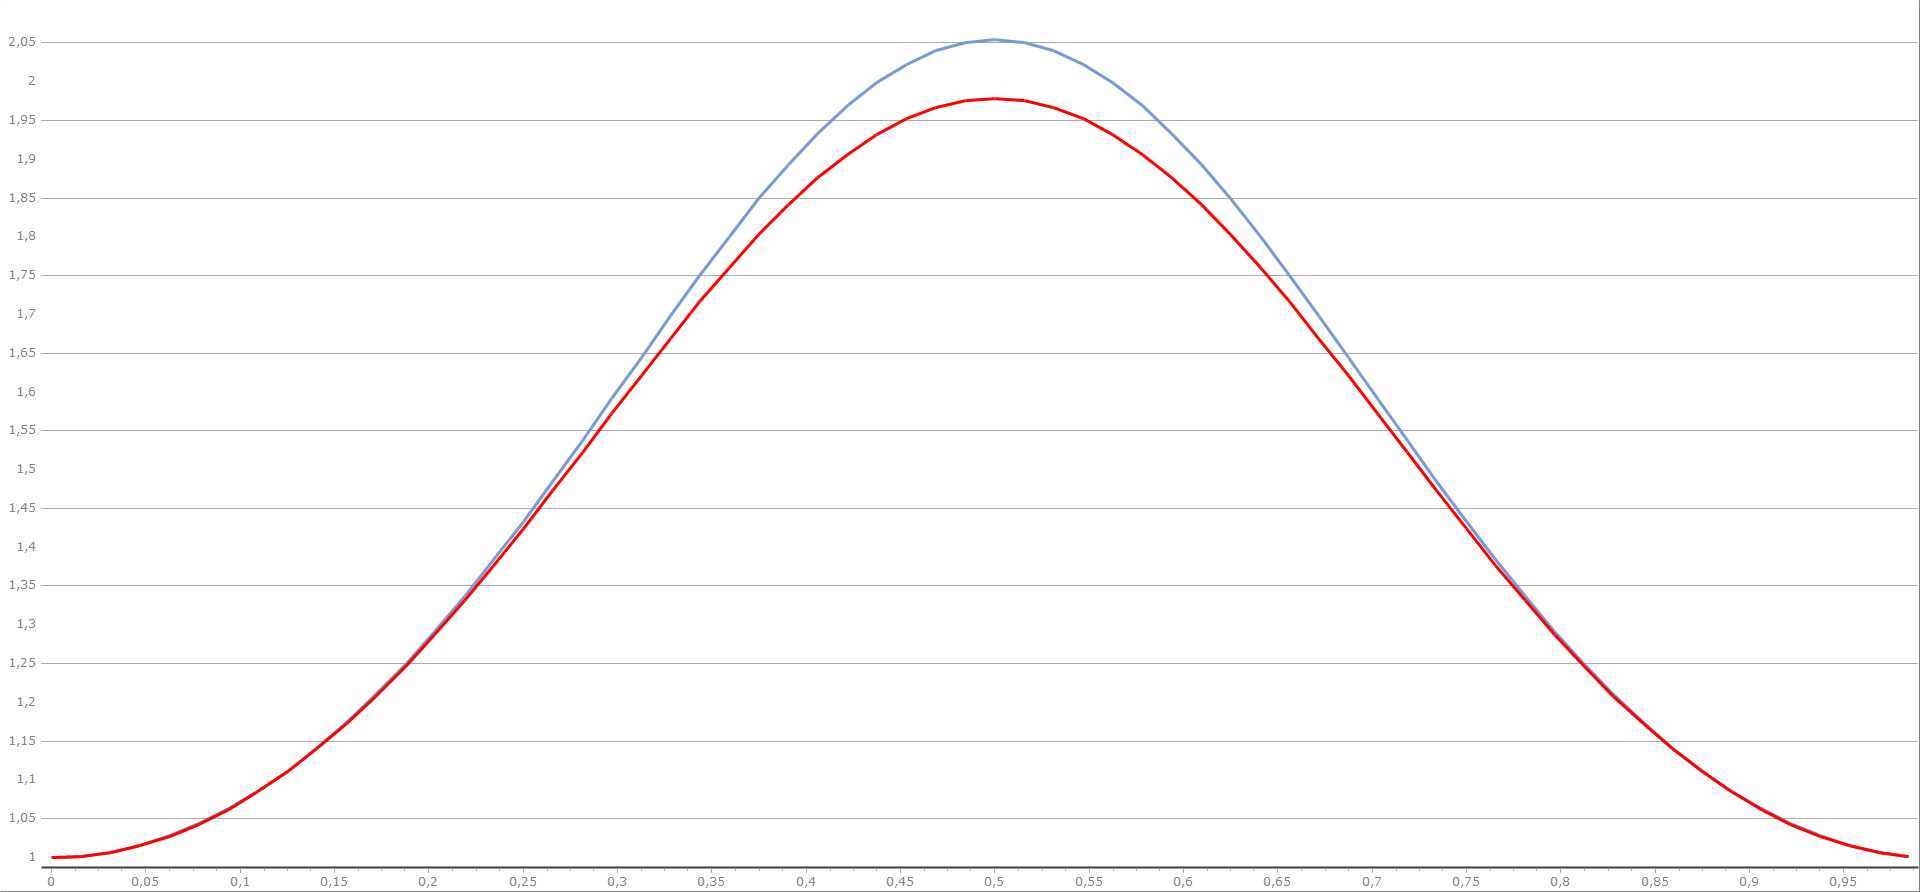
\includegraphics[width=.24\linewidth]{pictures/Ex1_image1_64(1)}
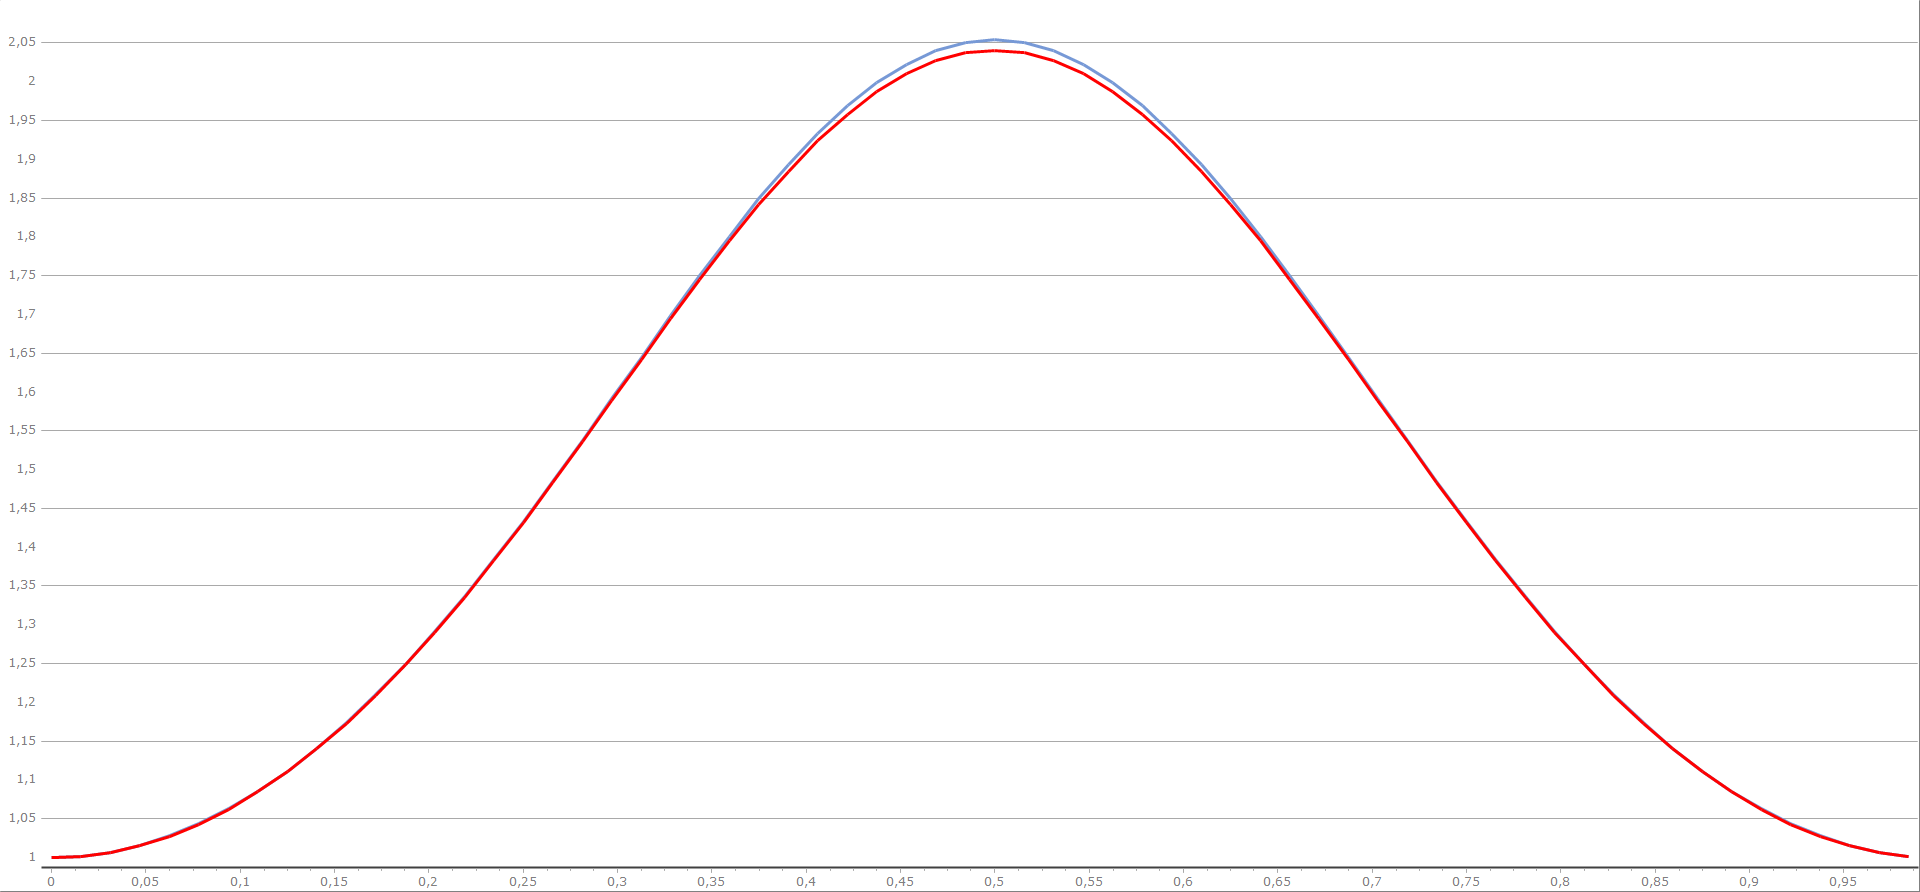
\includegraphics[width=.24\linewidth]{pictures/Ex1_image1_64(2)}
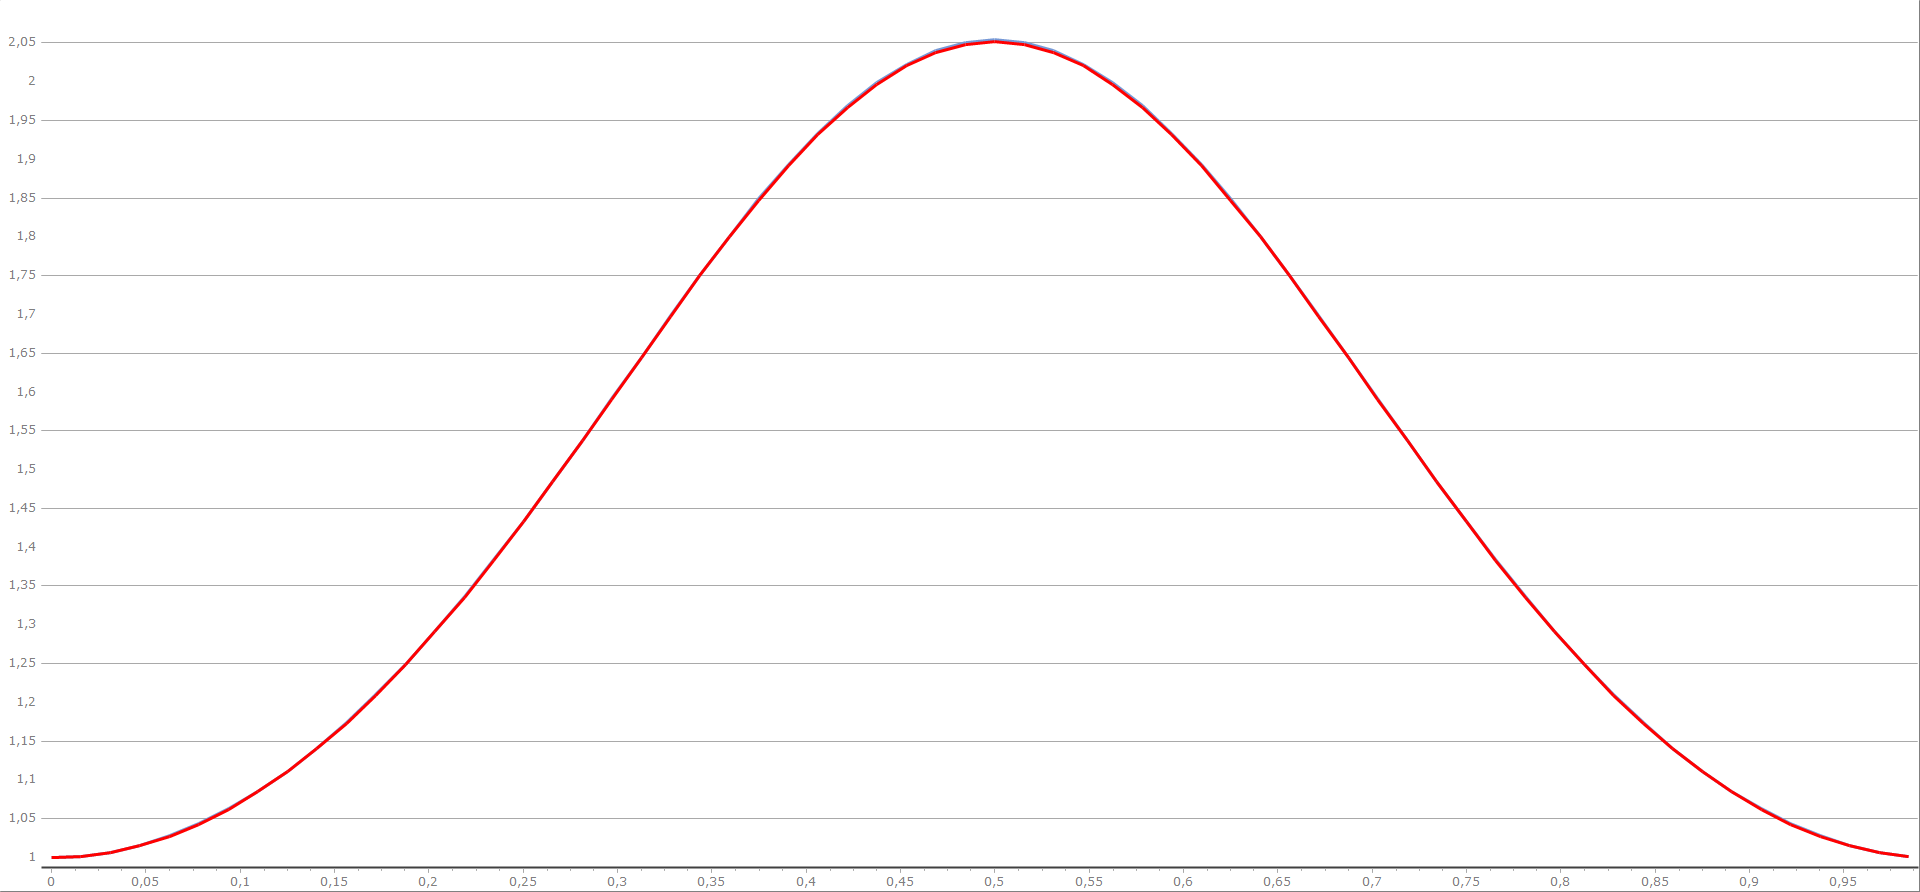
\includegraphics[width=.24\linewidth]{pictures/Ex1_image1_64(3)}
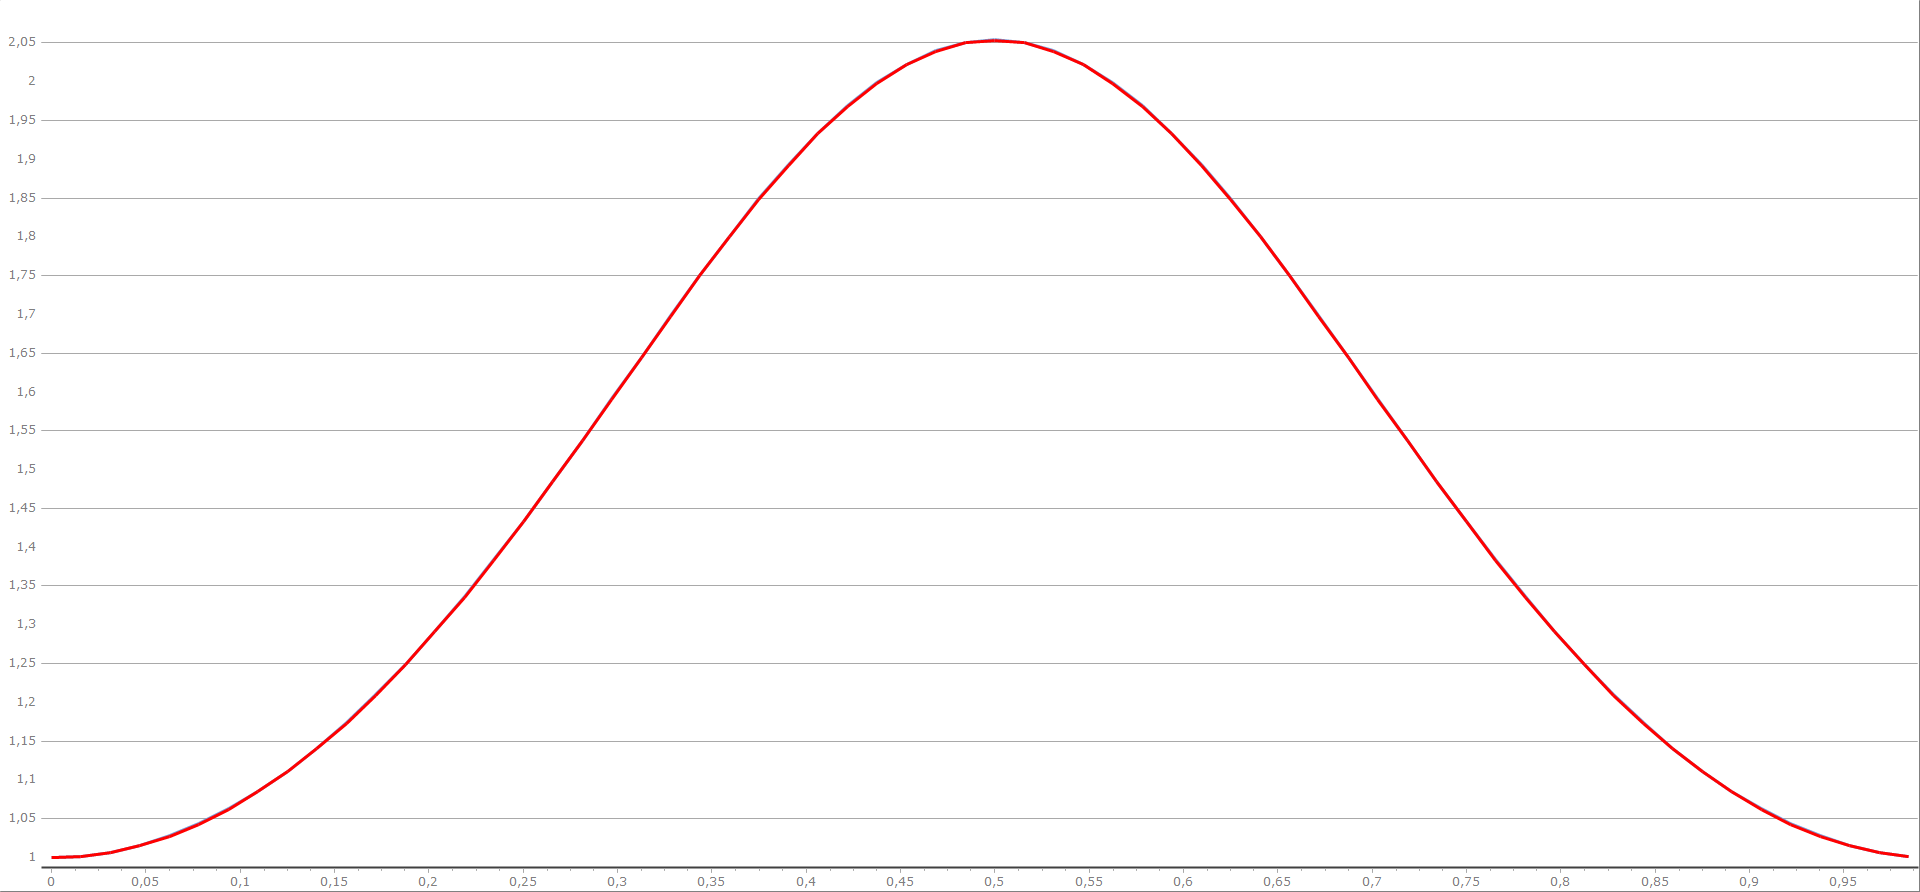
\includegraphics[width=.24\linewidth]{pictures/Ex1_image1_64(4)}
\caption{Первые 4 итерации применения программы к задаче \eqref{GasRamEx_Cou1} при $N=64$. Синим цветом обозначено точное решение, красным -- приближенное}
\label{pic1}
\end{figure}

\begin{example}
Решить задачу Коши
\begin{equation}\label{GasRamEx_Cou2}
y'=f(x,y),
\end{equation}
при
\begin{equation*}
f(x,y)=
\begin{cases}
\sqrt{1-y^2}\sin(x),\ |y|\leq 0,9,\\
\sqrt{1-0,9^2}\sin(x),\ y\in\mathbb{R}\setminus[-0,9;0,9],
\end{cases}
\quad y(0)=0, \quad 0\leq x\leq 1,5.
\end{equation*}
\end{example}
\textit{ Решение}. Точное решение этой задачи имеет вид: $y(x)=\sin(1-\cos(x))$. При $x=1,5\sin(\pi t)$, $\eta(t)=y(1,5\sin(\pi t))$ и с учетом того, что функция $\eta(t)$ симметрична относительно прямой $t=\frac12$, задача \eqref{GasRamEx_Cou2} примет следующий вид:
\begin{equation}\label{GasRamEx_Cou3}
\eta'(t)=1,5\cos(\pi t) \sin(1,5\sin(\pi t)) \sqrt{1-\eta^2(t)}, \quad \eta(0)=0, \quad 0\leq t\leq 1.
\end{equation}
На рисунке \ref{pic2} приведены первые 3 итерации применения программы к задаче \eqref{GasRamEx_Cou3} при $N=64$. Синим цветом обозначено точное решение, красным -- приближенное.
\begin{figure}
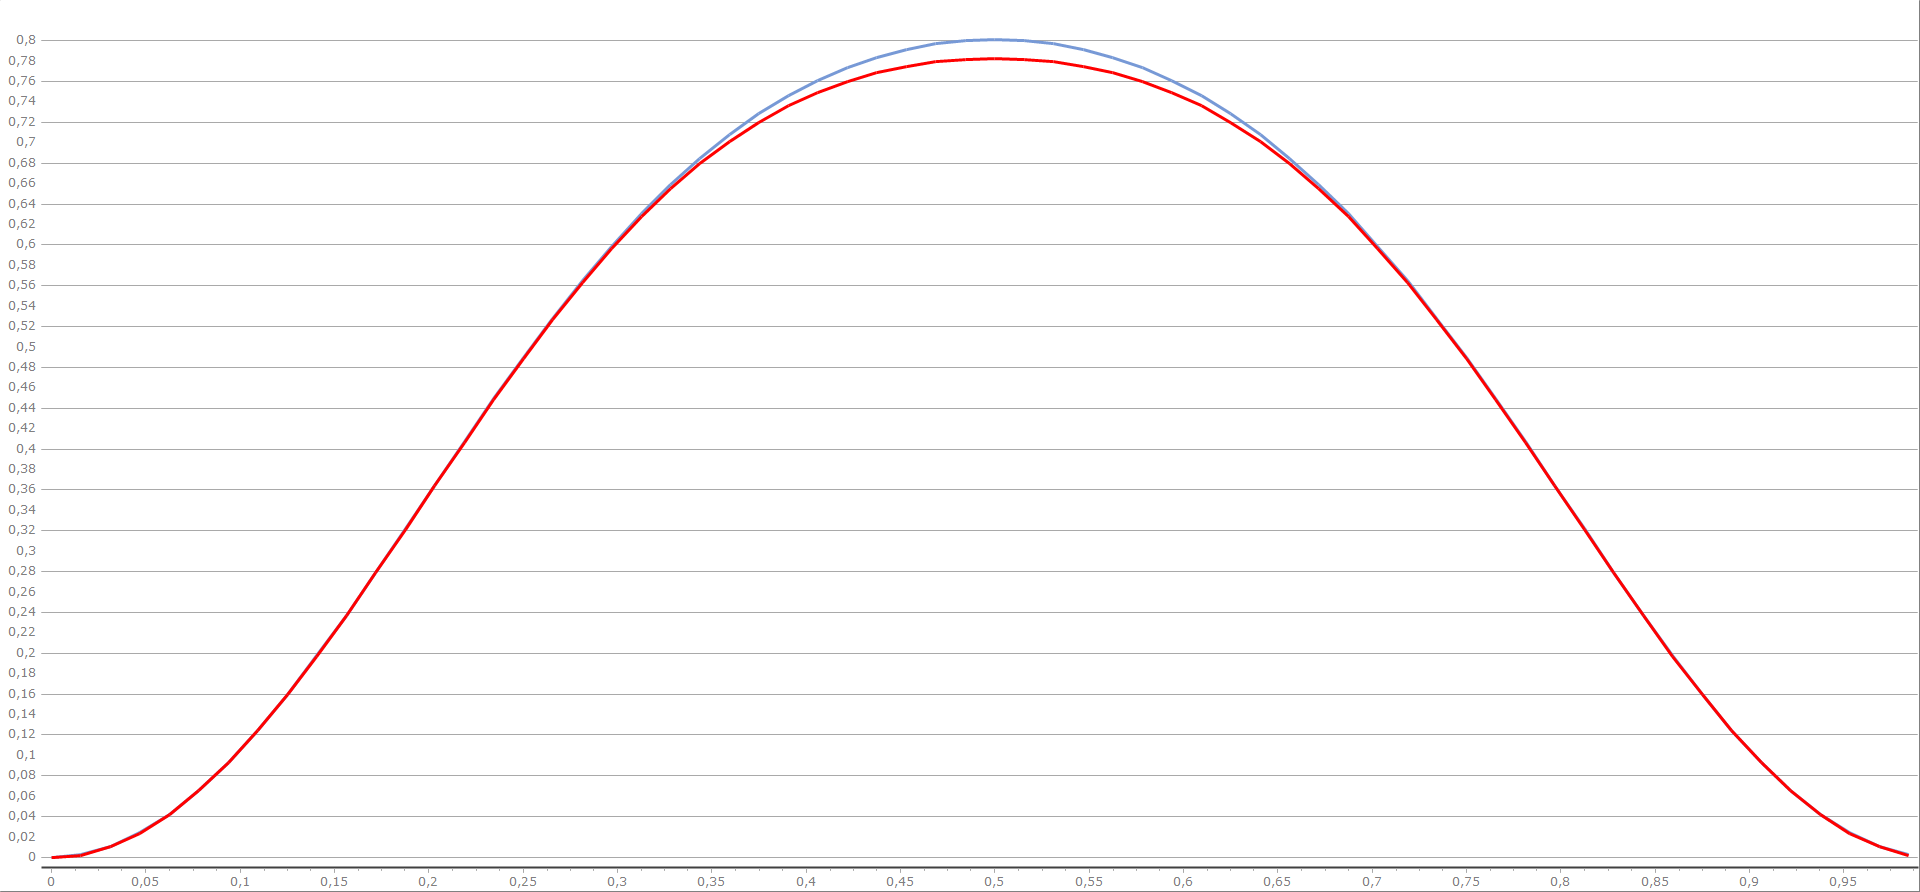
\includegraphics[width=.32\linewidth]{pictures/Ex2_image1_64(1)}
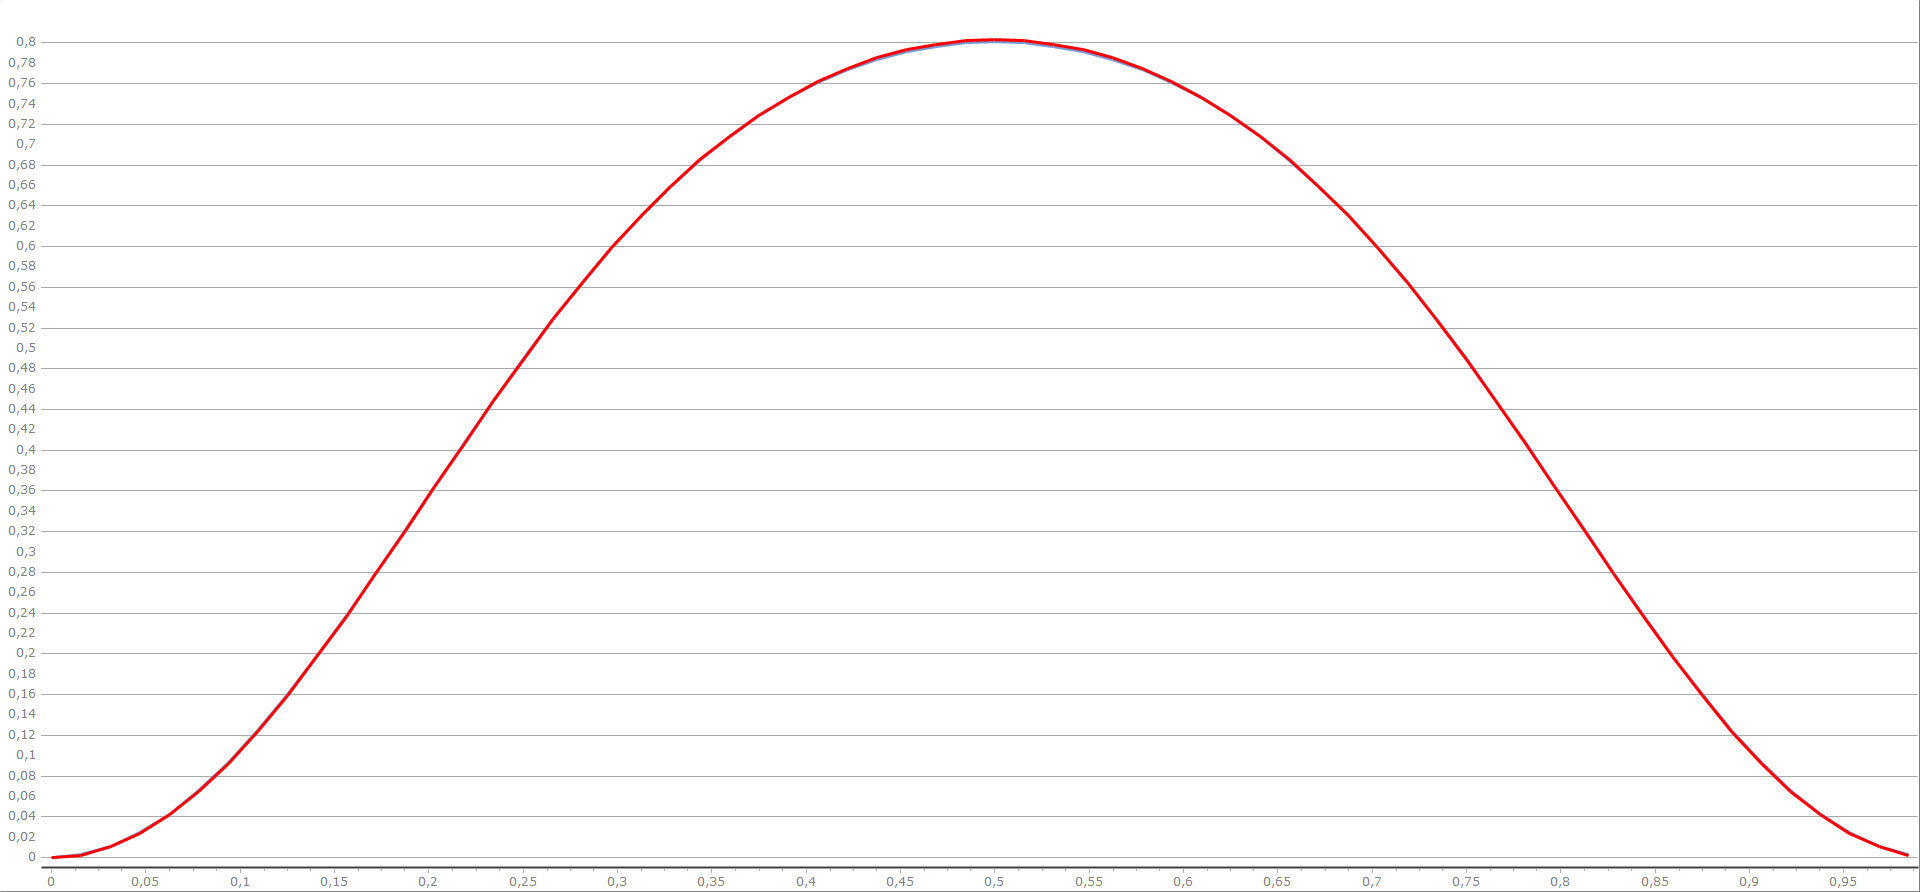
\includegraphics[width=.32\linewidth]{pictures/Ex2_image1_64(2)}
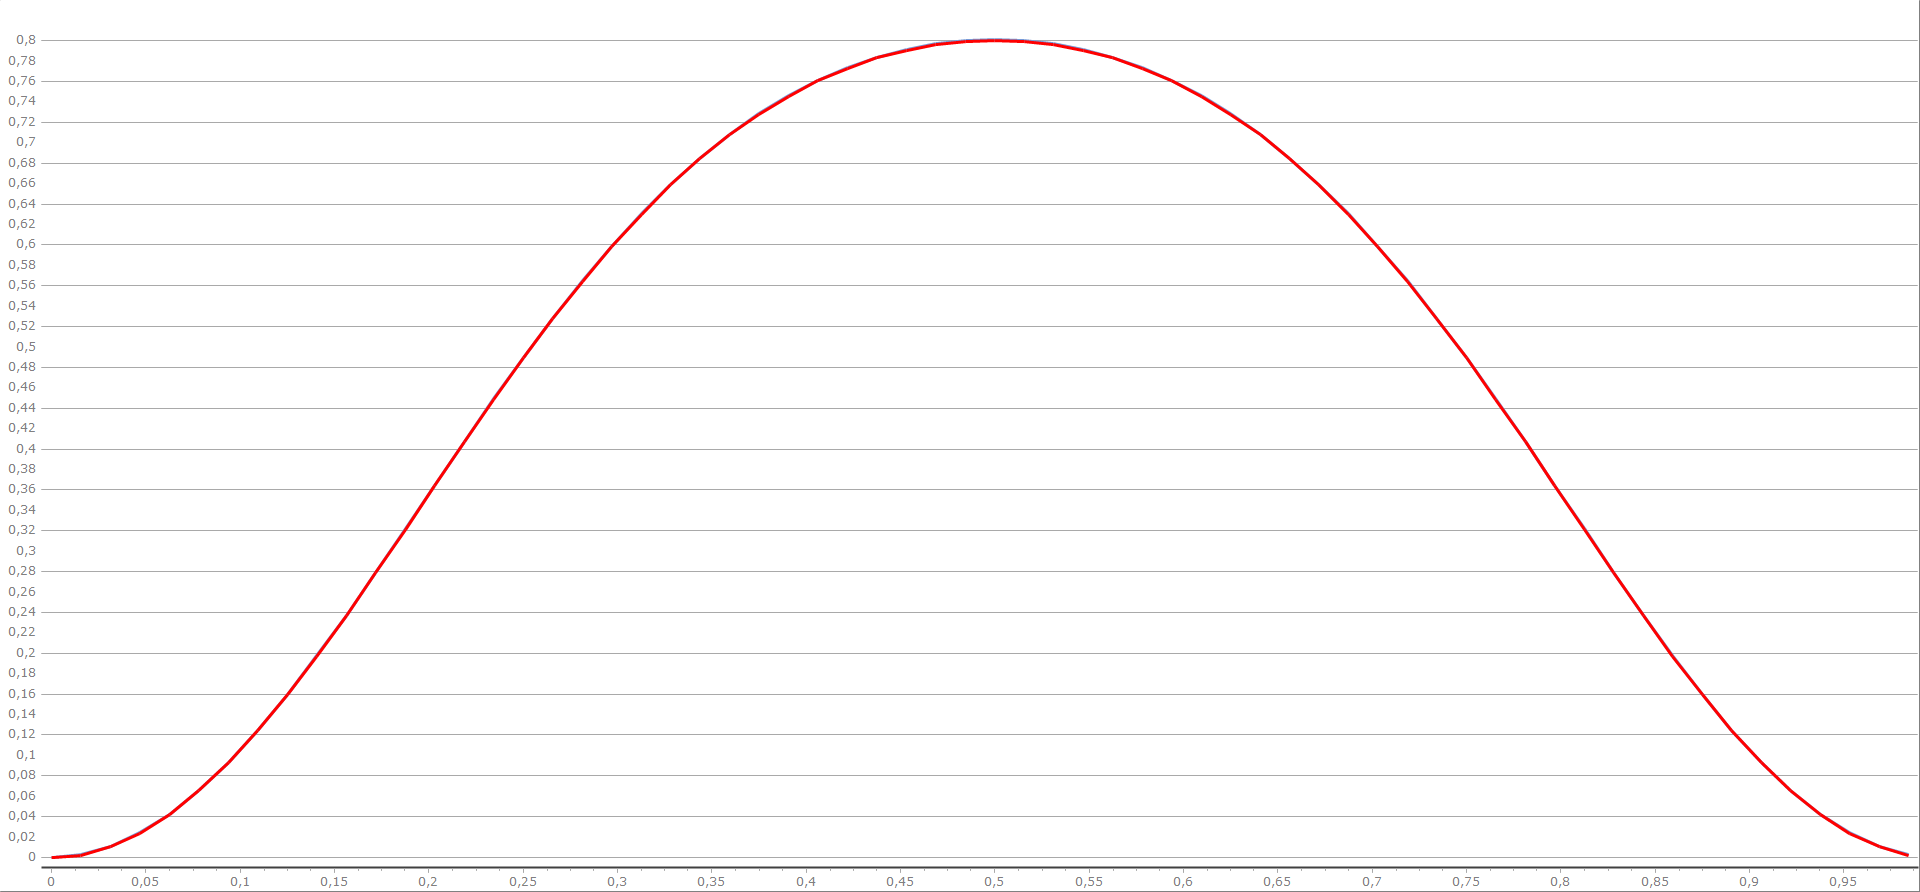
\includegraphics[width=.32\linewidth]{pictures/Ex2_image1_64(3)}
\caption{Первые 3 итерации применения программы к задаче \eqref{GasRamEx_Cou3} при $N=64$. Синим цветом обозначено точное решение, красным -- приближенное}
\label{pic2}
\end{figure}




%\subsection{Заключение}


%Программно реализован итерационный метод нахождения приближенного решения задачи Коши для ОДУ, путем вычисления коэффициентов разложения этого решения в ряд Фурье по функциям, ортонормированным
%относительно скалярного произведения Соболева и порожденным косинусами.
%Вычисление неизвестных коэффициентов осуществляется посредством применения алгоритма быстрого преобразования Фурье. Разработанная программа зарегистрирована в Роспатенте под названием <<Программа нахождения приближенного решения задачи Коши для ОДУ>>.



